\documentclass{beamer}

\mode<presentation>
{
  \usetheme{CambridgeUS}
  \setbeamercovered{transparent}
}

\usepackage[english]{babel}
\usepackage[latin1]{inputenc}
\usepackage{times}
\usepackage[T1]{fontenc} 
% Or whatever. Note that the encoding and the font should match. If T1
% does not look nice, try deleting the line with the fontenc.
\usepackage{amsmath}
\usepackage{algorithmic}

\newcommand{\linespace}{\vskip 0.25cm}

\definecolor{MyForestGreen}{rgb}{0,0.7,0} 
\newcommand{\tableemph}[1]{{#1}}
\newcommand{\tablewin}[1]{\tableemph{#1}}
\newcommand{\tablemid}[1]{\tableemph{#1}}
\newcommand{\tablelose}[1]{\tableemph{#1}}

\definecolor{MyLightGray}{rgb}{0.6,0.6,0.6}
\newcommand{\tabletie}[1]{\color{MyLightGray} {#1}}

% The text in square brackets is the short version of your title and will be used in the
% header/footer depending on your theme.
\title[Intrusion Detection]{Intrusion Detection with \\ Genetic Algorithms and Fuzzy Logic}

% Sub-titles are optional - uncomment and edit the next line if you want one.
% \subtitle{Why does sub-tree crossover work?} 

% The text in square brackets is the short version of your name(s) and will be used in the
% header/footer depending on your theme.
\author[Ireland]{Emma Ireland}

% The text in square brackets is the short version of your institution and will be used in the
% header/footer depending on your theme.
\institute[U of Minn, Morris]
{
  Division of Science and Mathematics \\
  University of Minnesota, Morris \\
  Morris, Minnesota, USA
}

% The text in square brackets is the short version of the date if you need that.
\date[December '13] % (optional)
{December 2013 \\ UMM CSci Senior Seminar Conference}

% Delete this, if you do not want the table of contents to pop up at
% the beginning of each subsection:
\AtBeginSection[]
{
  \begin{frame}<beamer>
    \frametitle{Outline}
    \tableofcontents[currentsection, hideothersubsections]
  \end{frame}
}

\begin{document}

\begin{frame}
  \titlepage
\end{frame}

% For a 20-25 minute senior seminar talk you probably want something like:
% - Two or three major sections (other than the summary).
% - At *most* three subsections per section.
% - Talk about 30s to 2min per frame. So there should probably be between
%   15 and 30 frames, all told.

\section*{Overview}

\subsection*{The big picture}

\begin{frame}
  \frametitle{The big picture}
  
  \begin{columns}
  \begin{column}{0.6\textwidth}
  \begin{itemize}
  	\item 
	\item 
	\item 
	\item 
	\item 
  \end{itemize}
  \end{column}
  \begin{column}{0.4\textwidth}
   
  \end{column}
  \end{columns}
\end{frame}

\subsection*{Outline}

\begin{frame}
  \frametitle{Outline}
  \tableofcontents[hideallsubsections]
\end{frame}
%%%%%%%%%%%%%%%%%%%%%%%%%%%%%%%%%%%%%%%%%%%%%%%%%%%%%%%%%%%%%%%%%%%%%%%%%%%%%%%%%
%%%%%%%%%%%%%%%%%%%%%%%%%%%%%%%%%%%%%%%%%%%%%%%%%%%%%%%%%%%%%%%%%%%%%%%%%%%%%%%%%
%%%%%%%%%%%%%%%%%%%%%%%%%%%%%%%%%%%%%%%%%%%%%%%%%%%%%%%%%%%%%%%%%%%%%%%%%%%%%%%%%
%%%%%%%%%%%%%%%%%%%%%%%%%%%%%%%%%%%%%%%%%%%%%%%%%%%%%%%%%%%%%%%%%%%%%%%%%%%%%%%%%
\section[Background]{Background}
\subsection{Types of Networking Attacks}
\begin{frame}
  \frametitle{title here}

\end{frame}


\subsection{Detection Methodologies}
\begin{frame}
  \frametitle{title}

\end{frame}


\subsection{Data Sets}
\begin{frame}
  \frametitle{title}

\end{frame}


\subsection{Rules}
\begin{frame}
  \frametitle{title}

\end{frame}


\subsection{Fuzzy Logic}
\begin{frame}
  \frametitle{title}

\end{frame}


\subsection{Genetic Algorithm}
\begin{frame}
  \frametitle{title}

\end{frame}


\subsection{Determining the accuracy of an algorithm}
\begin{frame}
  \frametitle{title}

\end{frame}
%%%%%%%%%%%%%%%%%%%%%%%%%%%%%%%%%%%%%%%%%%%%%%%%%%%%%%%%%%%%%%%%%%%%%%%%%%%%%%%%%
%%%%%%%%%%%%%%%%%%%%%%%%%%%%%%%%%%%%%%%%%%%%%%%%%%%%%%%%%%%%%%%%%%%%%%%%%%%%%%%%%
%%%%%%%%%%%%%%%%%%%%%%%%%%%%%%%%%%%%%%%%%%%%%%%%%%%%%%%%%%%%%%%%%%%%%%%%%%%%%%%%%
%%%%%%%%%%%%%%%%%%%%%%%%%%%%%%%%%%%%%%%%%%%%%%%%%%%%%%%%%%%%%%%%%%%%%%%%%%%%%%%%%
\section[Genetic Algorithm Implementation]{Genetic Algorithm Implementation}
\subsection{Algorithm Overview}
\begin{frame}
  \frametitle{title here}

\end{frame}


\subsection{Experimental Design and Results}
\begin{frame}
  \frametitle{title}

\end{frame}
%%%%%%%%%%%%%%%%%%%%%%%%%%%%%%%%%%%%%%%%%%%%%%%%%%%%%%%%%%%%%%%%%%%%%%%%%%%%%%%%%
%%%%%%%%%%%%%%%%%%%%%%%%%%%%%%%%%%%%%%%%%%%%%%%%%%%%%%%%%%%%%%%%%%%%%%%%%%%%%%%%%
%%%%%%%%%%%%%%%%%%%%%%%%%%%%%%%%%%%%%%%%%%%%%%%%%%%%%%%%%%%%%%%%%%%%%%%%%%%%%%%%%
%%%%%%%%%%%%%%%%%%%%%%%%%%%%%%%%%%%%%%%%%%%%%%%%%%%%%%%%%%%%%%%%%%%%%%%%%%%%%%%%%
\section[Fuzzy Genetic Algorithm Implementation]{Fuzzy Genetic Algorithm Implementation}

\subsection{Fuzzy Algorithm}

\begin{frame}
  \frametitle{Measuring the probability of a record being an attack}

  \begin{columns}
  \begin{column}{0.4\textwidth}
  \begin{itemize}
  	\item Trapezoidal shape
  \end{itemize}
  
  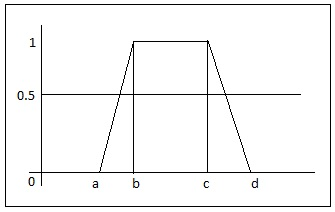
\includegraphics[width=0.95\textwidth]{../trapFigure.jpg}
  
  \begin{itemize}
	\item The parameters are the values of a feature.
  \end{itemize}  
  
  \end{column}


  \begin{column}{0.6\textwidth}
  \begin{itemize}
  	\item Fuzzy algorithm
  \end{itemize}
  
\begin{algorithmic}
\IF{data value is between $b$ and $c$}
  \STATE{prob = 1.0}
\ELSIF{data value is between $a$ and $b$}
  \STATE{
    prob = $(\textrm{data}-a)/(b-a)$
  }
\ELSIF{data value is between $c$ and $d$}
  \STATE{
    prob = $(d-\textrm{data})/(d-c)$
  }
\ELSE \STATE{prob = 0.0}
\ENDIF
\end{algorithmic}

  \end{column}
  \end{columns}
\end{frame}


\begin{frame}
	\frametitle{Encoding of features and rules}
	\begin{itemize}
	\item The four parameters are encoded into blocks.
	\item Each block is a feature with values between 0.0 and 7.0.
	\end{itemize}
	
\begin{figure}
\begin{tabular}{|cccc|} \hline
010 & 011 & 100 & 101\\
a=2 & b=3 & c=4 & d=5\\
\hline\end{tabular}
\end{figure}

	\begin{itemize}
	\item A rule has 12 blocks of features, at the end is the type of attack.
	\end{itemize}

\begin{figure}
\begin{tabular}{|cccc|c|cccc|c|} \hline
010 & 011 & 100 & 101   & ...... & 010 & 011 & 101 & 111   & DoS\\
a=2 & b=3 & c=4 & d=5   & ...... & a=2 & b=3 & c=5 & d=7   &\\ 
    &     & Block 1&    &        &     & Block 12& &       & Type\\
\hline\end{tabular}
\end{figure}

\end{frame}


\subsection{Algorithm Overview}

\begin{frame}
	\frametitle{title}
	
\end{frame}


\subsection{Experimental Design and Results}

\begin{frame}
	\frametitle{title}
	
\end{frame}
%%%%%%%%%%%%%%%%%%%%%%%%%%%%%%%%%%%%%%%%%%%%%%%%%%%%%%%%%%%%%%%%%%%%%%%%%%%%%%%%%
%%%%%%%%%%%%%%%%%%%%%%%%%%%%%%%%%%%%%%%%%%%%%%%%%%%%%%%%%%%%%%%%%%%%%%%%%%%%%%%%%
%%%%%%%%%%%%%%%%%%%%%%%%%%%%%%%%%%%%%%%%%%%%%%%%%%%%%%%%%%%%%%%%%%%%%%%%%%%%%%%%%
%%%%%%%%%%%%%%%%%%%%%%%%%%%%%%%%%%%%%%%%%%%%%%%%%%%%%%%%%%%%%%%%%%%%%%%%%%%%%%%%%
\section[Conclusions]{Conclusions}

\begin{frame}
\frametitle{Conclusions}

\begin{itemize}
  \item 
  
  \linespace
  
  \item 

  \linespace
  
  \item
\end{itemize}


\end{frame}

\begin{frame}
	\frametitle{Thanks!}
	
	Thank you for your time and attention!
		
	\linespace
	\linespace
	
	\begin{center}
	{\huge Questions?}
	\end{center}
\end{frame}

\section*{References}

\begin{frame} 
	\frametitle{References} 
	
	\begin{thebibliography}{lskdjf}
	
  	\end{thebibliography}
	
\end{frame} 

\end{document}


